\documentclass[11pt]{article}
\usepackage{geometry} % see geometry.pdf on how to lay out the page. There's lots.
\usepackage{hyperref}
\usepackage{graphicx}
\usepackage{gensymb}
\usepackage[affil-it]{authblk}
\usepackage[toc,page]{appendix}
\usepackage{pifont}
\usepackage{amsmath}
\usepackage{amsthm}
\usepackage{amsfonts}
\usepackage{hyperref}

\usepackage{float}

\newtheorem{theorem}{Theorem}
\newtheorem{corollary}{Corollary}

\newcommand\numberthis{\addtocounter{equation}{1}\tag{\theequation}}


\usepackage{draftwatermark}



\SetWatermarkText{DRAFT}
\SetWatermarkScale{6}
\SetWatermarkLightness{0.95}

% \geometry{letter} % or letter or a5paper or ... etc
% \geometry{landscape} % rotated page geometry

% See the ``Article customise'' template for come common customisations

\title{Untwisting the Tetrahelix (v0.12)}
\author{Robert L. Read \texttt{read.robert@gmail.com} \and
  Robert Gatliff \texttt{robert@toubat.org}
}


\date{\today}

%%% BEGIN DOCUMENT
\begin{document}

\maketitle

%% \tableofcontents

\begin{abstract}
  The Boerdijk--Coxeter helix (BC helix, or tetrahelix) is a
  face-to-face stack of regular tetrahedra.  Considering the edges of
  these tetrahedra as structural members, the resulting structure is attractive and
  inherently rigid, and therefore interesting to architects,
  mechanical engineers, and robotocists.  A formula is developed that matches the
  visually apparent helices forming the outer rails of the BC helix.
  This formula is generalized to a formula convenient to designers.
  Formulae for 
  computing the
  parameters that give edge-length minimax-optimal tetrahelices
  are given, defining a continuum of tetrahelices of varying curvature.
  The endpoints of the optimality of this continuum are the BC helix and
  a structure of zero curvature, the \emph{equitetrabeam}.
  Numerically finding the rail angle from the equation for
  pitch allows optimal tetrahelices of any pitch to be designed. 
  An interactive tool for such design and experimentation is provided: \url{https://pubinv.github.io/tetrahelix/}.
  A formula for the inradius of optimal tetrahelices is given.
  Utility for static and variable geometry
  truss/space frame design and robotics is discussed.
\end{abstract}


\section{Introduction}

The Boerdijk--Coxeter helix\cite{coxeter1985simplicial} (BC helix), is
a face-to-face stack of tetrahedra that winds about a straight axis.
Because architects, structural engineers, and robotocists are inspired
by and follow such mathematical models but can build structures and
machines of differing or even dynamically changing length, it is
useful to develop the mathematics of structures formed from tetrahedra
where we relax regularity.


The vertices of the tetrahedra lie upon
three helices about the central axis.  The
Tetrobot/Glussbot\cite{TetrobotBook} project uses the regularity of
this geometry to make a tentacle-like robot that can crawl like a slug
or mollusc.  The Tetrobot concept is to use mechanical members, called
actuators, which can change their length, connected by special joints,
such as the three-d printable Song-Kwon-Kim\cite{song2003spherical} joint, or the CMS joint\cite{HamlinSandersonCMS}
which allow many members to come to a single point.
Such machines can
follow purely regular mathematical models such as the Boerdijk–-Coxeter
helix or the Octet Truss\cite{richard1961synergetic}.

Buckminster Fuller called the BC helix a \emph{tetrahelix}\cite{fuller1982synergetics},
a term now commonly used. In this paper we reserve \emph{BC helix} to mean the purely regular structre and use \emph{tetrahelix} to refer
to any structure isomorphic to a the BC helix.



\begin{figure}[H]
  \centering
     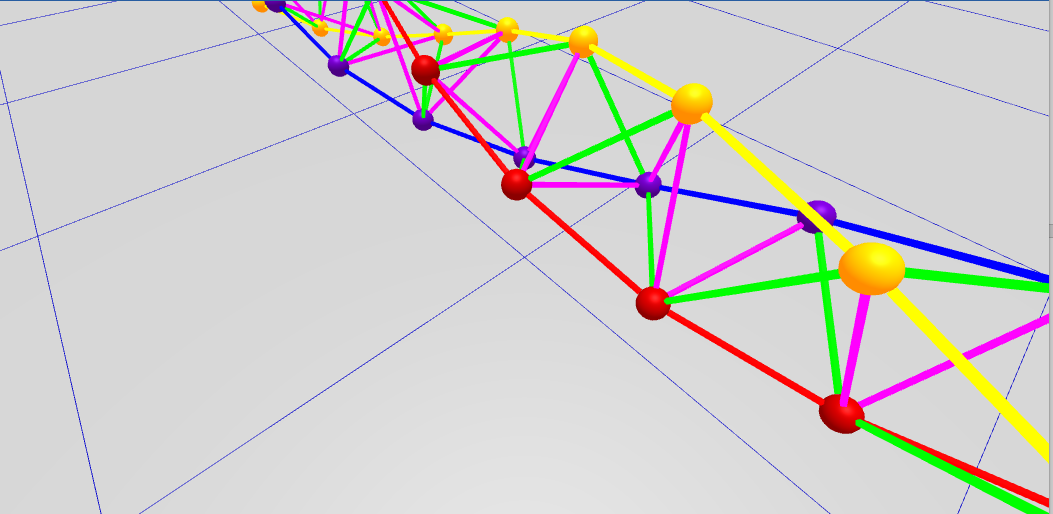
\includegraphics[width=0.95\textwidth]{figures/BCHelixCloseUp.png}
     \caption{BC Helix Close-up (partly along axis)}
  \centering
     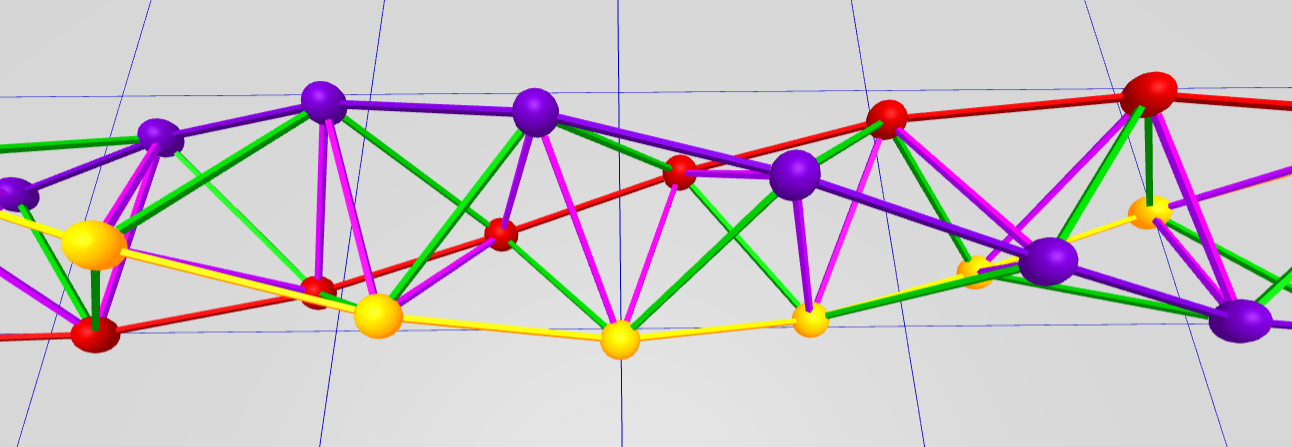
\includegraphics[width=0.95\textwidth]{figures/VerticalCloseUp.png}
     \caption{BC Helix Close-up (orthogonal)}
  \label{fig:closeup}
\end{figure}



Imagining Figure \ref{fig:closeup} as a static mechanical structure,
we observe that it is useful to the mechanical engineer or
robotocist because the structure remains an inherently rigid,
omni-triangulated space frame, which is
somewhat mechanically strong.
Imagine further in Figure \ref{fig:closeup}, that each static edge was replaced with an
actuator that could dynamically become shorter or longer in response to electronic control,
and the vertices were a joint that supported sufficient angular displacement
for this to be possible. Such a machine is a Tetrobot\cite{TetrobotBook}.

A BC helix does not rest comfortably on a plane. It is convenient to
be able to ``untwist'' it and to form a tetrahelix space frame that has a
flat planar surface. By making length changes in a certain way, we can
untwist a tetrahelix to form a \emph{tetrabeam} which has planar faces
and has, for example, an equilateral triangular profile. This paper
develops the equations needed to untwist the tetrahelix. All math
deveoped here is available in JavaScript and demonstrated by an interactive
design website \url{https://pubinv.github.io/tetrahelix/}\cite{readtetrahelix},
from which Figures \ref{fig:closeup} and
the figure below are taken.

\begin{figure}
  \centering
     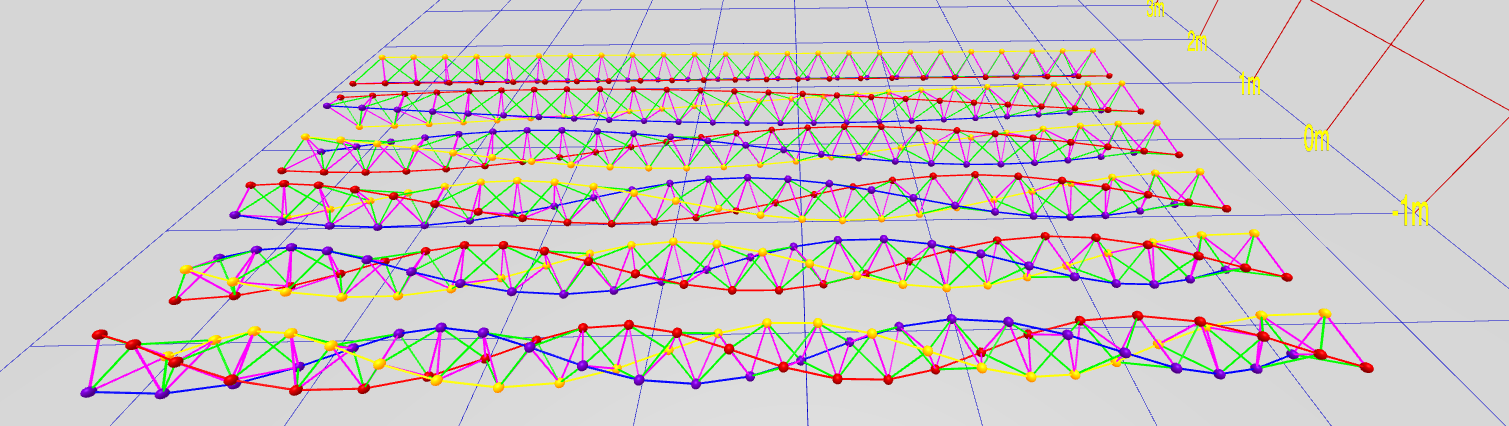
\includegraphics[width=0.95\textwidth]{figures/TetrahelixSeries.png}
     \caption{A Series of Tetrahelices}
  \label{fig:series}
\end{figure}


Figure \ref{fig:series} displays a continuum of tetrahelices optimal in a certain sense, which is the result of this
paper. The closest helix is the BC helix, and the furthest
is the equitetrabeam, defined in Section \ref{sec:equitetrabeam}.

\section{A Designer's Formulation of the BC Helix}

We would like to design nearly regular tetrahelices with a formula that
gives the vertices in space. Eventually we would like to design nearly regular
tetrahelices by choosing the lengths of a small set of members.
If you are designing a
space frame, this is a static design choice, in a robot, it is a
dynamic choice that can be used to twist\footnote{The formal definition of twistiness, or \emph{torsion},
  is not useful or used in the paper. The formal \emph{curvature} and \emph{torsion} of the helices defined here
may be easily computed from the formualae if desired.} the robot and/or exert linear or
angular force on the environment.

Ideally we would have a simple formula for defining the nodes based on
any curvature or pitch we choose. It is a goal of
this paper to relate these two approaches to generating a tetrahelix
continuum.


H.S.M Coxeter constructs the BC helix\cite{coxeter1985simplicial} as a repeated rotation and translation of the tetrahedra, showing the
rotation is:
\[
\theta = \arccos(-2/3) 
\]
and the translation:
\[
h_{bc} = 1/\sqrt{10}
\]

$\theta$ is approximately $131.81$ degrees.
The angle $\theta$ is the rotation of \emph{each} tetrahedra, not the tetraheda along a rail.  In Figure \ref{fig:closeup},
each tetrahedra has either a yellow, blue, or red outer edge or rail.
That is, a blue-rail tetrahedron is rotated slightly more than a $1/3$ of a revolution to match the face of the yellow tetrahedra.

R.W. Gray's site\cite{graytetrahelix}, repeating a formula by Coxeter\cite{coxeter1985simplicial} in more accessible form, gives the Cartesian coordinates $\begin{bmatrix}
           x \\
           y \\
           z
         \end{bmatrix}$
for a counter-clockwise BC Helix:
\begin{equation}
  \label{graycoxeter}
V(n) =
\left [
  \begin{tabular}{c}
   $ r_{bc} \cos{n \theta} $\\
   $ r_{bc} \sin{n \theta} $\\
   $ n h_{bc}  $
  \end{tabular}
  \right ],
\text{where:}
  \begin{tabular}{c}
 $ r_{bc} = \frac{3\sqrt{3}}{10} $\\
 $ h_{bc} = 1/\sqrt{10} $ \\
 $ \theta = \arccos(-2/3) $ \\
  \end{tabular}      
\end{equation}
where $n$ represents each integer numbered node in succession on every colored rail.

The apparent rotation of a vertex an outer-edge, $V(n)$ relative from $V(n+3)$ for any integer $n$
in \eqref{graycoxeter}, is $3 \theta - 2\pi$).

This formula defines a helix, but it is not any of the apparent helices, or rail helices, of the
BC helix, but rather one that winds three times as rapidly through all
nodes. To a designer of tetrahelices, it is more natural to think of
the three helices which are visually apparent, that is, those three
which are closely approximated by the outer edges or rails of
the BC helix. We think of each of these three rails as being a different color, red, blue, or yellow.

It is convenient to have a formula that gives us the nodes of just
one rail helix, denoted by color $c$:
\[
(\forall n \in \mathbb{Z}, \forall c \in \{0,1,2\} : H_{BCcolored}(n,c) = V(3n +c))
\]

Such a helix can be written:
\begin{equation}
  \label{eq:colored}
H_{BCcolored}(n,c) =
\left [
  \begin{tabular}{c}
   $ r_{bc}  \cos{((3 \theta - 2 \pi)n + c  \theta)} $\\
   $ r_{bc} \sin{((3 \theta - 2 \pi)n + c  \theta)} $\\
   $ 3 h_{bc} (n + c/3)  $
  \end{tabular}
  \right ],
\text{where:}
  \begin{tabular}{c}
 $ r_{bc} = \frac{3\sqrt{3}}{10} $\\
 $ h_{bc} = 1/\sqrt{10} $ \\
 $ \theta = \arccos(-2/3) $ \\
  \end{tabular}      
\end{equation}

In this formula, integral values of $n$ may be taken as a node number for one rail and used to compute its Cartesian
coordinates. Allowing $n$ to take non-integer values defines a continuous
helix in space which is close to the segmented polyline of the outer tetrahedra edges, and equals them at integer
values.

The quantity $ (3 \theta - 2 \pi) \approx 35.43 \degree $, and is the angular shift between $V(3n+c)=H_{BCcolored}(n,c)$ and
$V(3(n+1)+c)=H_{BCcolored}(n+1,c)$.
This quantity appears so often that we call it the ``rail angle rho''. For the BC helix, $\rho_{bc} = (3 \theta - 2 \pi)$.

\begin{figure}[H]
     \centering
     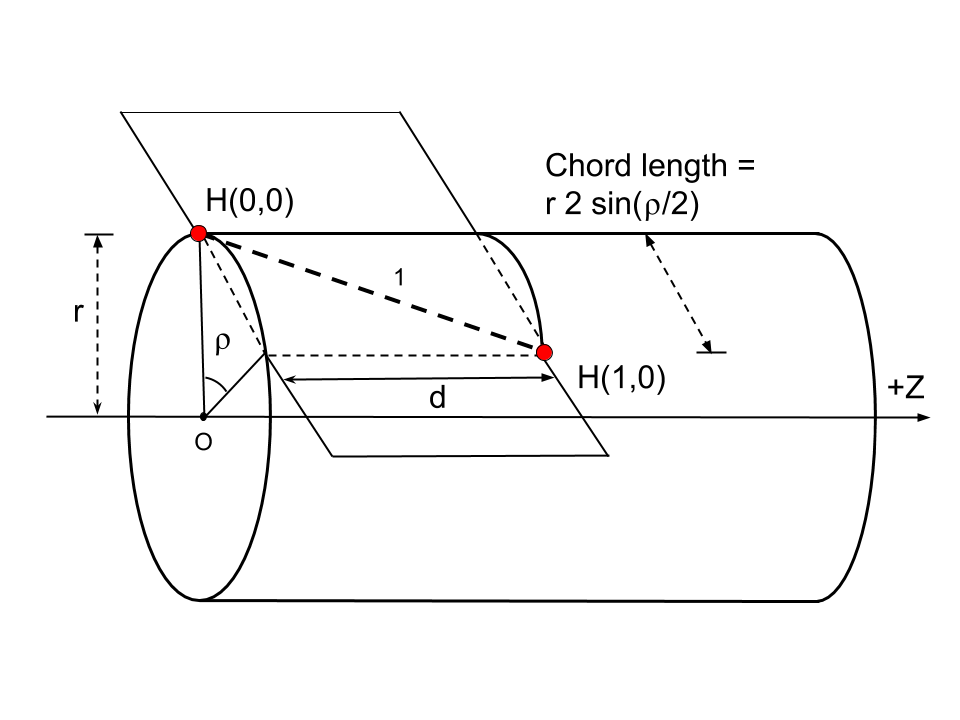
\includegraphics[width=0.7\textwidth]{figures/RailAngleGeometry.png}
     \caption{Rail Angle Geometry}
  \label{railanglefig}
\end{figure}

Note in Figure \ref{railanglefig} the $z$-axis travel for one rail edge is denoted by $d$. In \eqref{graycoxeter} and \eqref{eq:colored}, the variable
$h$ is used for one third of the distance we name $d$. We will later justify that $d = 3h$. In this paper we assume the length of a rail
is always $1$ is a simplification, although we make the rail length a parameter in our JavaScript code in \texttt{tetrahelixmath.js} \cite{readtetrahelix}.

The $H_{BCcolored}(n,c)$ formulation can be further clarified by rewriting directly in terms of the rail angle $\rho{bc}$ rather than $\theta$.
Intuitively we seek an expression where $c/3$ is multiplied by a $1/3$ rotation plus the rail angle $\rho$.
We expand 
the expressions $\theta$ and $\rho_{bc}$ in \eqref{eq:colored} and seek to isolate the term $c2\pi/3 $.
\begin{align*}
 c \theta  &=   \text{\{we aim for 3 in denominator, so we split...\}} \\
    (c/3)  (3 \theta)  &=   \text{\{we want $2\pi$ in numerator, so add canceling terms...\}} \\
 (c/ 3) ((3 \theta - 2 \pi)  + 2 \pi) &= \text{\{definition of $\rho_{bc}$\}...} \\  
  (c / 3) \rho_{bc}  + c 2 \pi /3 &=  \text{algebra...} \\  
c  ( \rho_{bc} +  2 \pi) /3  \\
\end{align*}

This allows us to redefine:

%% Actually, I am not sure if this is a clearer formulation...it might be, and need to put it in general!!!
\begin{equation}
H_{BCcolored}(n,c) =
\left [
  \begin{tabular}{c}
    $ r  \cos{\rho_{bc} n + c (\rho_{bc} +  2 \pi) /3} $\\
   $ r  \sin{\rho_{bc} n + c (\rho_{bc} +  2 \pi) /3} $\\
   $ (n+c/3)  h_{bc} $
  \end{tabular}
  \right ],
\text{where:}
  \begin{tabular}{c}
%%  $\kappa = n + c/3$ \\
    $\rho_{bc} = (3 \theta - 2 \pi)$ \\
    $ \theta = \arccos(-2/3) $ \\
    $ h_{bc} = 1/\sqrt{10} $ \\    
  \end{tabular}      
\end{equation}

Recall that $c \in \{0,1,2\}$, but $n$ is continuous (rational or real-valued.)

From this formulation it is easy to see that moving one vertex on a rail
($H_{BCcolored}(n,c)$ to $H_{BCcolored}(n+1,c)$ for any $n$ and $c$)
moves us $\rho_{bc}$ radians around a circle. Since:
\[ \frac{2 \pi}{\rho_{bc}} \approx 10.16
\]
we can see that there are approximately $10.16$ red, blue or yellow tetrahedra on one rail in a single revolution.

The pitch of the Boerdijk--Coxeter helix of edge length $1$ is the length of three tetrahedra times this number:
\begin{align*}
   \frac{3 h_{bc}\cdot  2 \pi }{\rho_{bc}} 
  &= \frac{6 \pi}{\sqrt{10}\rho_{bc}} 
  &\approx 9.64 
\end{align*}


The pitch is less than the number of tetrahedra because the tetrahedra
are not lined up perfectly.  It is a famous and interesting result
that the pitch is irrational. A BC helix never has two tetrahedra at
precisely the same orientation around the $z$-axis. However, this is
inconvenient to designers, who might prefer a rational pitch.
The idea of developing a rational period by arranging solid tetrahedra by relaxing the face-to-face matching
has been explored\cite{sadler2013periodic}. 
We develop below slightly irregular edge lengths that support, for example, a pitch of precisely 12
tetrahedra in one revolution which would allow an architect to design a
column having a basis and a capital in the same relation to the
tetrahedra they touch at the bottom and top of the column.


\section{Optimal Tetrahelices}

We use the term \emph{tetrahelix} to mean any structure made of
vertices and edges which is isomorphic to the BC helix, in which the
vertices lie on three helices. We further demand that all edge lengths
be finite, as we are only interested in physically constructable tetrahelices.
By isomporphic we mean there is a one-to-one mapping between both
vertices and edges in the two tetrahelices.
One could consider various definitions of optimality for a
tetrahelix, but the most useful to us as robotocists extending the Tetrobot concept is to minimize the
maximum difference between any two edges, because the Tetrobot uses linear acutators of limit range of extension.


If all three rails do not have the same pitch, there is an edge of
unbounded length, so it is hardly optimal. So we are justified in talking about the
\emph{pitch} of 
the tetrahelix as the pitch of its rail helices, even though there are
three such helices.

Similarly, if the axes are not parallel, there is an edge of
unbounded length in the structure, so we exclude such a strcturue.

Since the axes are parallel, we may define the \emph{inradius}, represented by the letter $i$, of a
tetrahelix to be the radius of the largest
cylinder parallel to this axis contained within the circumscribing cylinder
which is penetrated by no edge.
Define a \emph{minimax edge-length optimal tetrahelix} or just an
\emph{optimal tetrahelix} to be a tetrahelix for which there exists
no other tetrahelix of the same inradius and pitch with a lower maximum
difference between its edge lengths. 

We wish to show that in an optimal tetrahelix, all vertices lie on the cylinder
of radius $r$, regardless of where they lie on the $z$-axis.

Since all three rails have the same rail length, no matter how we
move the rails in the $xy$ plane if we shorten the $xy$ distance between
vertices we shorten the total distance.
Our tool for thinking about this is to project out the $z$ dimension to form
a two-dimensional figure of nodes and non-rail edges (see Figure \ref{untouchingrailfig}.)
Consider the projection along the $z$ axis of all vertices and non-rail edges into the $xy$ plane, which will be
a figure of dots and connecting segments in the $xy$ plane. The convex
hull for any one helix projection will be a circle (if its pitch is
irrational) or a polygon if rational, or a point if the helix has
zero curvature. Each of these figures by definitions lies outside the
circle of inradius $i$ in the $xy$ plane.

\begin{theorem}
  \label{thm:cylinder}
  Any optimal tetrahelix with a rail angle less than $\pi$ has all vertices on a single cylinder.
\end{theorem}

\begin{proof}

Case 1: Suppose that $\rho$ is zero. Then for any given inradius, an equilateral
triangle is the minimax solution for all non-rail edges. Since there is only
one rail-edge length, this is the minimax solution for the entire set. Since
the vertices of an equilateral triangle lies on a circle, all points lie on
a cylinder.

Case 2: Suppose that $\rho$ is positive but less than $\pi$.
In this case each rail helix has
curavature and places points on both sides of any line through the origin
of the $xy$ plane (or both coincident on such a line.)

We first show that the inradius is touched by one segment from each pair
of rails.

\begin{figure}[H]
     \centering
     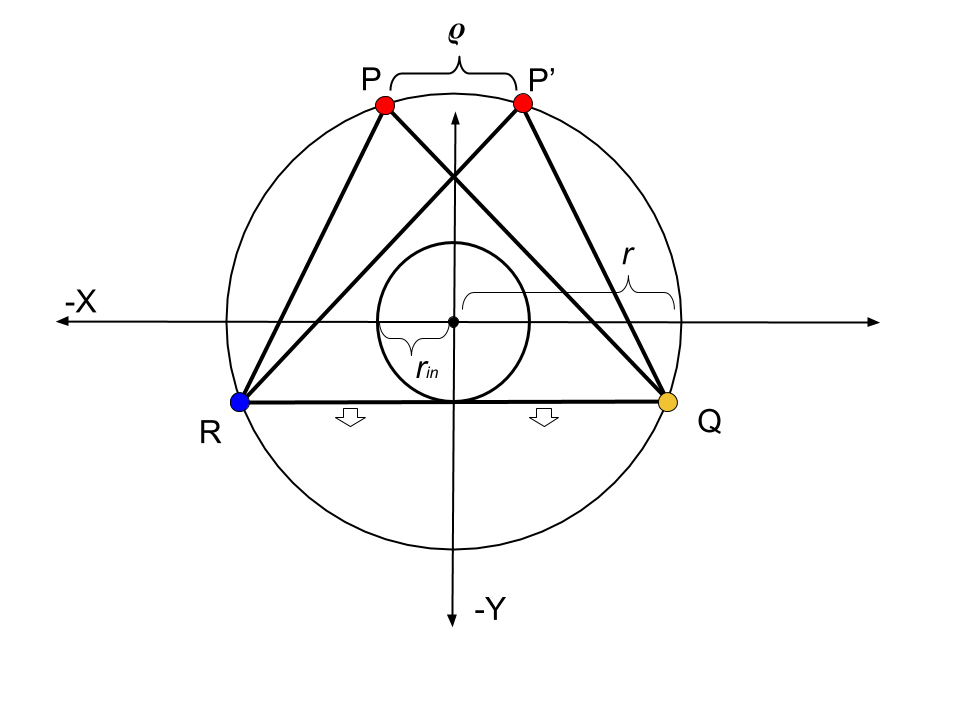
\includegraphics[width=0.7\textwidth]{figures/UntouchingRail.png}
     \caption{Untouching Rail}
  \label{untouchingrailfig}
\end{figure}

Figure \ref{untouchingrailfig} depicts a projection of
only the point $P$, the point $P'$ which is an adjacent vertex on the same rail,
and the intermediary points $R$ and $Q$ on the other two rails.

Supoose there is a rail $P$ which does not have a segment touching the incircle
at all in the projection, as depicted in Figure \ref{untouchingrailfig}.
Then a segment connecting the other two $Q$ and $R$ is a longest
rail, because any chord touching an incircle is longer than any which does not.
These two rails ($Q$ and $R$) can be moved closer to each other, and further away from $P$, to form a better minimax solution
by shortening the longest rail, until one of the segments from $P$ the previously
untouching rail touches one of the incircle. By induction, then all rails have
at least one segement touching each vertex on the rail that is tangent to the
incircle in an optimal tetrahelix.

Now suppose that you attempt to move the axis of one of the rails. Because
$\rho > 0 $ and $\rho$ is not a multiple of $\pi$, there is some vertex on the two sides of any diameter
halving our circle. Moving the axis of a tetrahelix lengthens a longest line while ``pinching'' the
inradius on the other side, so it is not optimal. Since the axes of these helices are the
same and they have the same curvature and pitch, the points defined by the helices all lie
on a cylinder.


\end{proof}

Theorem \ref{thm:cylinder} is not true when $\rho$ is an odd integer multiple of $\pi$.

Now that we have shown that any optimal tetrahelix vertices
are on helices of the same axes and pitch, we see that the vertices 
of any optimal tetrahelix will lie on a cylinder, or a circle when axis dimension
is projected out. Therefore it is reasonable to now speak of the \emph{radius} $r$
of a tetrahelix as the radius of the cylinder, as distinct from the inradius $i$.

Now that we have coincident axes, the same pitch, and the same radius, we can go on to
 the harder proof about where vertices occur along the $z$-axis.

 We show that in fact the nodes must be distributed in even thirds
 along the $z$-axis.

 Note that from the point of view of a single edge, we are on a
 slanted cylinder, when $\rho \neq 0$.  This means from its point of
 view a cross section is an ellipse. So we have to be very careful in
 comparing lengths of edges relative to the tetrahedron, because a
 change in position along the edge changes the length of a line, but
 in a complicated way depending on where it is relative to the
 ellipse.

 In principle in any 3 helices with the same axis of the same radius
 having any relative
 displacement along the $z$ axis there are 9 distinct edge classes.
 If when projecting all vertices on the the $z$-axis, the interval
 defined by the $z$ axis value of its endpoints contains no other vertices,
 we call it a \emph{one-hop} edge, and if it does contain another vertex we
 call it a \emph{two-hop} edge.
 Then there are 
 3 rail edges, 3 one-hop lengths between each pair of 3 rails, and 3 two hop
 lengths between each pair of three rails, where the two-hop length is at least
 the one-hop length.
 However, we have already shown the rail
 lengths are equal in any optimal tetrahelix.

\begin{theorem}
  \label{eventhirds}
  An optimal tetrahelix of any rail angle $\rho < \pi$ has all nodes evenly spaced at $d/3$ intervals on the $z$ axis.
  Any one tetrahedron in a tetrahelix has $1$ rail edge, $2$ one-hop edges connected to the rail and $2$ two-hop edges connected to the rail.
  The edge opposite of the rail edge is a one-hop edge.
\end{theorem}

\begin{proof}
    Consider the tetrahelix in which the vertices are evenly spaced at
    $h/3$ intervals on the $z$ axis. Every edge is either a rail edge,
    or it makes one hop, or it makes two hops. All of the one-hop
    edges are equal length.  All of the two-hop edges are equal
    length.

    Every vertex is connected to 4 non-rail edges. There is a one-hop edge
    in both the positive and negative $z$ direction. Likewise there is a two-hop
    edge in both the positive and negative $z$ direction. Let $A$ be the set
    of edge lengths, which has only 3 members, represented by $A = \{o,t,r\}$ for
    the one-hop, two-hop, and rail edge lengths.

    Any attempt to move any rail in either $z$ direction lengthens one two-hop edge to $t'$, where $t' > t$
    edge and shortens one one-hop edge $o' < o$. Let $B = \{o',t' \} \cup A$ be new edges.
    The minimax of $B$ is greater than the minimax of $A$ since there is a single rail length which cannot be both greater
    than $t'$ and $o'$ and less than $t'$ and $o'$.
    Therefore, any optimal tetrahelix has all one-hop edges between all rails are equal to each other, and
    all two-hop edges are equal to each other, and the $z$ distances between rails are equal, and therefore
    $d/3$ from each other.
\end{proof}

 Note that based on Theorem \ref{eventhirds}, there are only 3 possible lengths in an optimal tethrahelix,
 and we are justified in classifying edge lengths as \emph{rail}, \emph{one-hop}, or
\emph{two-hop}. The one-hop edges are the edges between closest on the $z$-axis, and the two-hop edges are those that skip over a vertex.

By Theorem \ref{eventhirds} every optimal tetrahelix has vertices lying on helices expressible in the form:
\[
V_{optimal}(n,c) =
\left [
  \begin{tabular}{c}
   $ r \cos(n \alpha +  c 2 \pi /3)$\\
   $ r \sin(n \alpha +  c 2 \pi /3) $\\
   $ \frac{d(n +c / 3)}{3}   $
  \end{tabular}
  \right ],
\text{where:}
\begin{tabular}{c}
  $c \in \{0,1,2\}$
  \end{tabular}      
\]
where we have not yet investigated in the general case the relationships beteween $\alpha$, $r$, and $d$ in this formulation.
However, we understand that when $\alpha = 0$, the helices are degenerate, having curvature of $0$, and
we have the equitetrabeam.




\section{Parameterizing Tetrahelices via Rail Angle}

We seek a formula to generate optimal tetrahelices that accepts a
parameter that allows us to design the tetrahelix conveniently.
Please refer back to Figure \ref{railanglefig}.
The pitch of the helix is an obious choice, but is not defined when the
curvature is $0$, an important special case. The radius or the axial
distance between two nodes on the same rail are obvious choices, but
perhaps the clearest choice is to build formula that takes as its
input the ``rail angle'' $\rho$. We define $\rho$ to be the angle
formed in the X,Y plane $\angle A O B$ projecting out the $z$
axis and sighting along the positive $z$ axis. In other words, $\rho$
controls how far a rail edge of a tetrahelix deviates from being
parallel with the axis, or the ``twistiness'' of tetrahelix. We use
the parameter $\chi = 1$ to indicate a chirality or counter-clockwise,
and $\chi = -1$ for clockwise.



 These quantities are related by the expression:

\begin{align*}
  1^2 &= d^2 + (2 r \sin{ \rho / 2})^2 \\
%%  1 &= d^2 + 4 r^2 (\sin{ \rho / 2})^2 \\
  d^2 &= 1 - 4 r^2 (\sin{ \rho / 2})^2    \numberthis  \label{railangle} \\
\end{align*}

Checking the important special case of the BC helix, we find that this equation
indeed holds true (treating $d$ in this equation as $3 h_{bc}$ as defined by
Gray and Coxeter, that is, $d_{bc} = 3h_{bc}$, where they are using it for the axial height from one node to
the next of a different color, but we use it to mean distance for the same color.

The rail angle $\rho$ also has the meaning that $2 \pi / \rho$ is the number of
tetraheda in a full revolution of the helix.

In choosing $\rho$, one greatly constrains $r$ and $d$, but does not completely
determine both of them together, so we treat both as parameters.

Rewriting our formulation in terms of $\rho$:
\begin{equation}
  \label{eq:general}
H_{general}(\chi,n,c,\rho,d_{\rho},r_{\rho}) =
\left [
  \begin{tabular}{c}
   $ r_{\rho} \cos(\chi \cdot (n \rho + c(\rho +  2 \pi) /3)) $\\
   $ r_{\rho}  \sin(\chi \cdot (n \rho + c(\rho +  2 \pi) /3)) $\\
   $ d_{\rho} (n + c /3) $
  \end{tabular}
  \right ],
\text{where:}
\begin{tabular}{c}
  $   1 = d_{\rho}^2 + 4 r_{\rho}^2 (\sin{ \rho / 2})^2 $ \\
%%  $\kappa = n + c/3$ \\
    $\chi \in \{-1,1\}$ \\  
  \end{tabular}      
\end{equation}


$H_{general}$ forces the user to select three values: $\rho$, $r_{\rho}$, and $d_{\rho}$ satisfying \eqref{railangle}.

Note that when $\rho = 0$ then $h_{\rho} = 1$, but $r_{\rho}$ is not determined by
Equation \ref{railangle}.

\begin{theorem}
  \label{generalformulaoptimal}
  The tetrahelices generated by $H_{general}$ are optimal in terms of minimum maximum member length when $r_{\rho}$ is chosen so that
  the length of the one-hop edge is equal to the rail length.
\end{theorem}


\begin{proof}
This is proved by a minimax argument.

By Theoerm \ref{eventhirds}, we can compute the (at most) three edge-lengths of an optimal
tetrahelix by formula universally quantified by $n$ and $c$:
\begin{align*}
  \text{rail} &= dist(H_{general}(n,c,\rho,d_{\rho},r_{\rho}),H_{general}(n+1,c,\rho,d_{\rho}),r_{\rho})) = 1 \\
  \text{one-hop} &= dist(H_{general}(n,c,\rho,d_{\rho},r_{\rho}),H_{general}(n,c+1,\rho,d_{\rho},r_{\rho}))  \\
  \text{two-hop} &= dist(H_{general}(n,c,\rho,d_{\rho},r_{\rho}),H_{general}(n,c+2,\rho,d_{\rho},r_{\rho}))  \\  
\end{align*}
where $dist$ is the Cartesian distance function.

\begin{align*}
  \text{one-hop} &= dist(H_{general}(n,c,\rho,d_{\rho}),H_{general}(n,c+1,\rho,d_{\rho}),r_{\rho})  \\
%%  \text{one-hop} &= dist(H_{general}(0,0,\rho,d_{\rho}),H_{general}(0,1,\rho,d_{\rho},r_{\rho}))  \\  
%%  \text{one-hop}  &= \sqrt{\frac{d_{\rho}^2}{9} + (r_{\rho}\sin(0) - r_{\rho}\sin(\rho/3+1\cdot\frac{2\pi}{3}))^2  +
%%    (r_{\rho}\cos(0) - r_{\rho}\cos(\rho/3 + 1\cdot\frac{2\pi}{3}))^2} \\
%%  \text{one-hop}  &= \sqrt{\frac{d_{\rho}^2}{9} + (0  - r_{\rho}\sin(\rho/3 + \frac{2\pi}{3}))^2  +
%%    (r_{\rho} - r_{\rho}\cos(\rho/3 + \frac{2\pi}{3}))^2} \\
%%  \text{one-hop}  &= \sqrt{\frac{d_{\rho}^2}{9} + r_{\rho}^2\sin^2(\rho/3 + \frac{2\pi}{3})  +
%%    r_{\rho}^2(1 - \cos(\rho/3 + \frac{2\pi}{3}))^2} \\
  %% Formula above checks at sqrt(8/27), 1, 0, and rho_bc, h_bc, r_bc.
  \text{one-hop}  &= \sqrt{\frac{d_{\rho}^2}{9} + r_{\rho}^2(\sin^2(\rho/3 + \frac{2\pi}{3})  + (1 - \cos(\rho/3 + \frac{2\pi}{3}))^2)} \\
  \text{but: }  d_{\rho}^2 &= 1 - 4 r_{\rho}^2 (\sin( \rho / 2)^2 \text{ ...so we substitute:}\\
  %% Formula above checks at sqrt(8/27), 1, 0, and rho_bc, h_bc, r_bc.  
  \text{one-hop}  &= \sqrt{\frac{1}{9}  + r_{\rho}^2(-\frac{4 (\sin^2( \rho / 2))}{9} + \sin^2(\rho/3+ \frac{2\pi}{3})  + (1 - \cos(\rho/3 + \frac{2\pi}{3}))^2)} \\
  %% Formula above checks at sqrt(8/27), 1, 0, and rho_bc, h_bc, r_bc.    
\end{align*}

By similar algebra and trigonometry:
\begin{align*}
  \text{two-hop}  &= \sqrt{\frac{4}{9} + r_{\rho}^2 (-\frac{16 (\sin^2( \rho / 2))}{9} + \sin^2(2\rho/3 + \frac{4\pi}{3})  + (1 - \cos(2\rho/3 + \frac{4\pi}{3}))^2)} \\
\end{align*}

We would really like to know the partial derivative of the two-hop - one-hop with respect
to the radius to be able to understand how to choose the radius to form the minimimax optimum.

Let:
\begin{equation}
  f_{\rho} = -\frac{4 (\sin^2( \rho / 2))}{9}
  \end{equation}
\begin{equation}
  g_{\rho} = -\frac{16 (\sin^2( \rho / 2))}{9} 
\end{equation}

\begin{equation}
  j_{\rho} = \sin^2(\rho/3+ \frac{2\pi}{3})  + (1 - \cos(\rho/3 + \frac{2\pi}{3}))^2)
\end{equation}
\begin{equation}
  k_{\rho} = (\sin^2(2\rho/3 + \frac{4\pi}{3})  + (1 - \cos(2\rho/3 + \frac{4\pi}{3}))^2)
\end{equation}

Then:
\begin{align*}
  \text{two-hop} - \text{one-hop}  &= \sqrt{\frac{4}{9}  + r_{\rho}^2(g_{\rho}+ j_{\rho})}
  - \sqrt{\frac{1}{9} +r_{\rho}^2(f_{\rho}+k_{\rho}) }
\end{align*}



By graph inspection using Mathematica, we see the partial derivative of this with respect to
radius $r_{\rho}$ is always negative.
Since the partial derivative of $\text{two-hop} - \text{one-hop}$ with respect to the
radius $r_{\rho}$ is negative up until $\rho_{bc}$ where it is $0$, 
we opitmize the overall minimax distance by choosing the largest radius
up until one-hop $= 1$, the rail-edge length.

Therefore we decrease the minimax length
of the whole system as we increase the radius
up unto the point that the shorter, one-hop distance is equal to the rail-length ($1$).
Therefore, to optimize the whole system so long as $\rho \leq \rho_{bc}$,
we equate one-hop to $1$ to find the optimum radius:


\begin{align*}
  1 &=  \sqrt{\frac{1}{9}  + r_{opt}^2(-\frac{4 (\sin^2( \rho / 2))}{9} + \sin^2(\rho/3+ \frac{2\pi}{3})  + (1 - \cos(\rho/3 + \frac{2\pi}{3}))^2)} \\
  r_{opt} &= \frac{2}{\sqrt{\frac{9}{2} \cdot ( \sqrt{3} sin(\rho/3) + \cos(\rho/3)) + \cos(\rho)+ 8 }} \numberthis  \label{eqrhoopt} \\
\end{align*}

We can now give a formula for $ d_{opt} $ computed from $\rho, r_{opt}$ via the rail angle equation \eqref{railangle}:

\begin{align*}
  d_{opt}^2 &= 1 - 4 \frac{2}{\sqrt{\frac{9}{2} \cdot ( \sqrt{3} \sin(\rho/3) + \cos(\rho/3)) + \cos(\rho)+ 8 }}^2 (\sin{ \rho / 2})^2   \\
%%  d_{opt}^2 &= 1 - 4 \frac{4(\sin{ \rho / 2})^2}{\frac{9}{2} \cdot ( \sqrt{3} \sin(\rho/3) + \cos(\rho/3)) + \cos(\rho)+ 8 }    \\
  d_{opt}^2 &= 1 - \frac{16(\sin{ \rho / 2})^2}{9 ( \sqrt{3} \sin(\rho/3) + \cos(\rho/3)) + \cos(\rho)+ 8 }    \\
%%  d_{opt}^2 &= 1 - \frac{16 \sin^2(\rho / 2) }{ \cos(\rho) + 9( \sqrt{3} \sin(\rho/3) + \cos(\rho/3)) + 8 }   \\
    d_{opt} &= \sqrt{1 - \frac{16 \sin^2(\rho / 2) }{ \cos(\rho) + 9( \sqrt{3} \sin(\rho/3) + \cos(\rho/3)) + 8 }}    \numberthis  \label{dopt}  \\      
\end{align*}

Thus, by computing $r_{opt}$  and $d_{opt}$ as a function of $\rho$ from this equation, we can construct minimax optimal tetrahelix for an $0 \leq \rho \leq \rho_{bc}$.
\end{proof}

If you look down the axis of an optimal tetrahelix, it happens that only one of the one-hop edges
comes closest to the axis. In other words, they define the radius of the incircle of the
projection, or the radius of a cylinder that would just fit inside the tetrahelix.
This is useful to know if the tetrahelix is used as a structure to house a pipe or
a ladder that must bear a human or to armor a conduit. The inradius $i_\rho$ of
an optimal tetrahelix is a remarkably simple function of the radius $r$ and the rail angle $\rho$:
\begin{equation}
  \label{eq:inradius}
  i_{\rho} = r \sin{\frac{\pi - \rho}{6}}
\end{equation}
Which can be seen from the trigonometry of a diagram of the projected one-hop edges
connecting four sequentially numbered vertices:

\begin{figure}[H]
  \label{projectiondiagram}
     \centering
     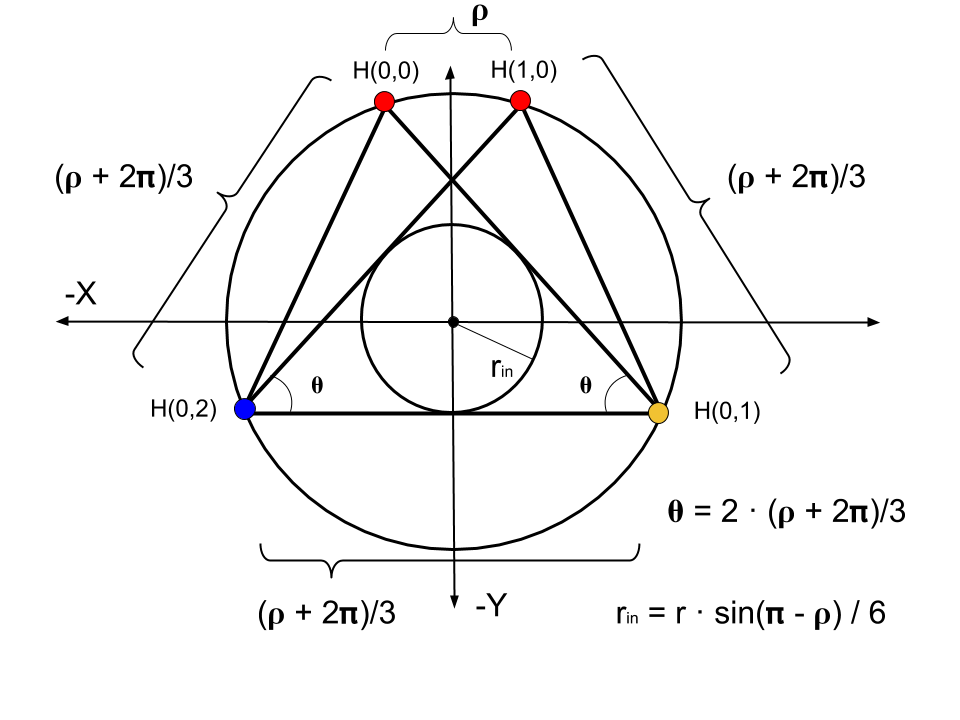
\includegraphics[width=0.8\textwidth]{figures/ProjectionDiagram.png}
     \caption{General One-hop Projection Diagram}
\end{figure}

From this equation with the help of symbolic computation we observe that inradius of the BC helix of unit rail length is $i_{\rho_{bc}} = \frac{3}{10\sqrt{2}} \approx 0.21213$.

\section{The Equitetrabeam}
\label{sec:equitetrabeam}

Just as $H_{general}$ constructs the BC helix (with careful and non-obvious choices of parameters)
which is an important
special case due to its regularity, it constructs an additional special
(degenerate) case when the rail angle $\rho = 0$
and $d = 1$ (the edgelength), where the cross sectional area is
an equilateral triangle of unchanging orientation.
We call this the \emph{equitetrabeam}.


\begin{corollary}
  The equitetrabeam with minimal maximal edge difference is produced
  by $H_{general}$ when $ r = \sqrt{\frac{8}{27}} $.
\end{corollary}

\begin{proof}
Choosing $d = 1$ and $\rho = 0$ we use Equation \eqref{eqrhoopt} to find the radius of 
optimal minimax difference.

Substituting into \eqref{eq:general}:

\begin{align*}
  \text{one-hop} &= \sqrt{\frac{1}{9} + 3r^2}\\
\end{align*}
Then:
\begin{align*}
   1  &=  \sqrt{\frac{1}{9} + 3r^2} & \text{ solved by... }\\
   r  &= \sqrt{\frac{8}{27}} &\approx 0.5443 \\
\end{align*}
\end{proof}

This radius\footnote{Another interesting but non-optimal solution is derived by setting
  (one-hop + two-hop)/2 = 1,
  occurs at $r = \sqrt{35}/4$ which produces
  three length classes of $11/12, 12/12, 13/12$.}
produces a two-hop rail length of $\frac{2}{\sqrt{3}}$.
The difference between this and $1$ is $\approx 15.47\% $. The inradius if the equitetrabeam of unit
rail length from both Equation \eqref{eq:inradius} and the fact that the inradius of
an equilateral triangle is half the circumradius is $\sqrt{\frac{8}{27}}/2$, or $\frac{\sqrt{6}}{9}$.




\begin{figure}[H]
     \centering
     \includegraphics[width=0.6\textwidth]{figures/EquitetrabeamUnfolded.JPG}
     \caption{Projection Diagram}
  \label{fig:unfolded}
\end{figure}

In Figure \ref{fig:series}, the furthest tetrahelix is the optimal equitetrabeam.
Figure \ref{fig:unfolded} shows a representation of an unfolded equitetrabeam.
Note that folding the outer edges of the paper upward or downward effectively
chooses the chirality of the equitetrabeam.

To the extent that we value tetrabeams (that is, tetrahelicies with a rail angle of $0$,
and therefore zero curvature) as mathematical or engineering objects
we have motivated the development of $H_{general}$ as a transformation of $V(n)$ defined by
Equation \eqref{graycoxeter} from Gray and Coxeter, as it is difficult to see how
the $V(n)$ 
formulation could ever give rise to a continuum producing the tetrabeam,
since setting the angle in that equation to zero can produce only collinear points.

Note that the equitetrabeam has chirality, which becomes important in our attempt to build a
continuum of tetrahelices.

\section{An Untwisted Continuum}


We observe that Equations \eqref{eqrhoopt} and \eqref{dopt} compute $r_{opt}$ and $d_{opt}$ which
create an optimal tetrahelix for any value rail angle $\rho$ between $0$, which
gives the equitetrabeam and
$\rho_{bc} \approx 35.43 \degree$, which gives the BC helix.

 Because the equitetrabeam which has a rail angle of $0$ still has
 chirality, that is, one still must decide to connect the one-hop edge to
 the clockwise or the counter-clockwise node, it is not poosible to build
 a smooth continuum where $\rho$ transitions from positive to negative
 which remains optimal. One can use a negative $\rho$ in $H_{general}$
 but it does not produce minimax optimal tetrahelices. In other words,
 untwisting a conter-clockwise tetrahelix to rail angle $0$ and then going
even further does produce a clockwise tetrahelix, but one in which the
 one-hop and two-hop lengths in the wrong places (that is, two-hop
 becomes shorter than one-hop.) Likewise, $\rho > \rho_{bc}$ generates
 a tetrahelix, but minimax optimality is not guaranteed by $H_{general}$.
 
The pitch of any tetrahelix 
where $\rho \neq 0$ is:
\begin{equation}
  \label{pitcheqn}
p(\rho) = \frac{2 \pi  \cdot d}{\rho}
\end{equation}
For a fixed $z$-axis travel $d$, this is trivial.
However, if one is computing 
$z$-axis travel from \eqref{dopt} the pitch is not simple.
It increases monotonically and smoothly with decreasing $\rho$, so
Equation \eqref{pitcheqn} can be easily solved numerically with a Newton-Raphson
solver, as we do on our website.
For a pitch at least $ p \geq \frac{3  \sqrt{2}  \pi}{\sqrt{5}\rho_{bc}} \approx 9.64 $,
using \eqref{dopt} produces minimax optimal tetrahelices.

In this way a rail angle can be chosen for any desired (sufficiently large) pitch, yield
the optimum radius, one-hop, and two-hop lengths an engineer needs to
construct a physical structure.

Perhaps surprisingly, the optimal untwisting is accomplished only by
changing the length of the two-hop member, leaving the one-hop member
and rail length equivalent within this continuum.\footnote{Before deriving Equation \eqref{eqrhoopt}, we created a continuum by
using a linear interpolation between the optimal radius for the
Equitetrabeam and the BC Helix. This minimax optimum of this simpler
approach was at most 1\% worse than the optimum computed by
\eqref{eqrhoopt}.}
 However, it should
be noted that an engineer or architect may also use $H_{general}$
directly and interactively, and that minimax length optimality is a
mathematic starting point rather than the final word on the beauty and utility of
physical structures. For example, a structural engineer might increase
radius in order to resist buckling. If an equitetrabeam were actually
used as a beam, an engineer might start with the optimal tetrabeam and
dilate it in one dimension to ``deepen'' the beam. Similarly, simple
changes curve the equitetrabeam into an ``arch''.

Trusses and space frames remain an important design field in
mechanical and structural engineering\cite{mikulas1985sequentially},
including deployable and moving trusses\cite{claypool2012readily}.


\section{Utility for Robotics}

Starting twenty years ago, Sanderson\cite{sanderson1996modular},
Hamlin,cite{TetrobotBook}, Lee\cite{lee2002dynamic}, and others
 created a style of robotics based on changing
the lengths of members joined at the center of a joint, thereby
creating a connection to pure geometry. More recently NASA has
experimented with tensegrities\cite{NTRT}, a different point in the
same design spectrum. These fields create a need to explore the notion
of geometries changing over time, not generally considered directly by
pure geometry.

As suggested by Buckminster Fuller, the most convenient geometries to
consider are those that have regular member lengths, in order to
facilitate the inexpensive manufacture and construction of the robot.
In a plane, the octet truss\cite{richard1961synergetic} is such a geometry, but in a line, the
Boerdijk--Coxeter helix is a regular structure.

However, a robot must move, and so it is interesting to consider the
transmutations of these geometries, which was in fact the motivation
for creating the equitetrabream.

\begin{theorem}
  By changing only the length of the longer members that connect two distinct rails (the two-hop members), you can dynamically untwist a tetrobot
  forming the Boerdijk-Coxeter configuration to the equitetrabeam which rests flat on the plane.
\end{theorem}

\begin{proof}
  Proof by our computer program that does this using Equation \eqref{eq:general} applied to the
  7-tet Tetrobot/Glussbot.

\begin{figure}[H] %float with two figures
  \centering
     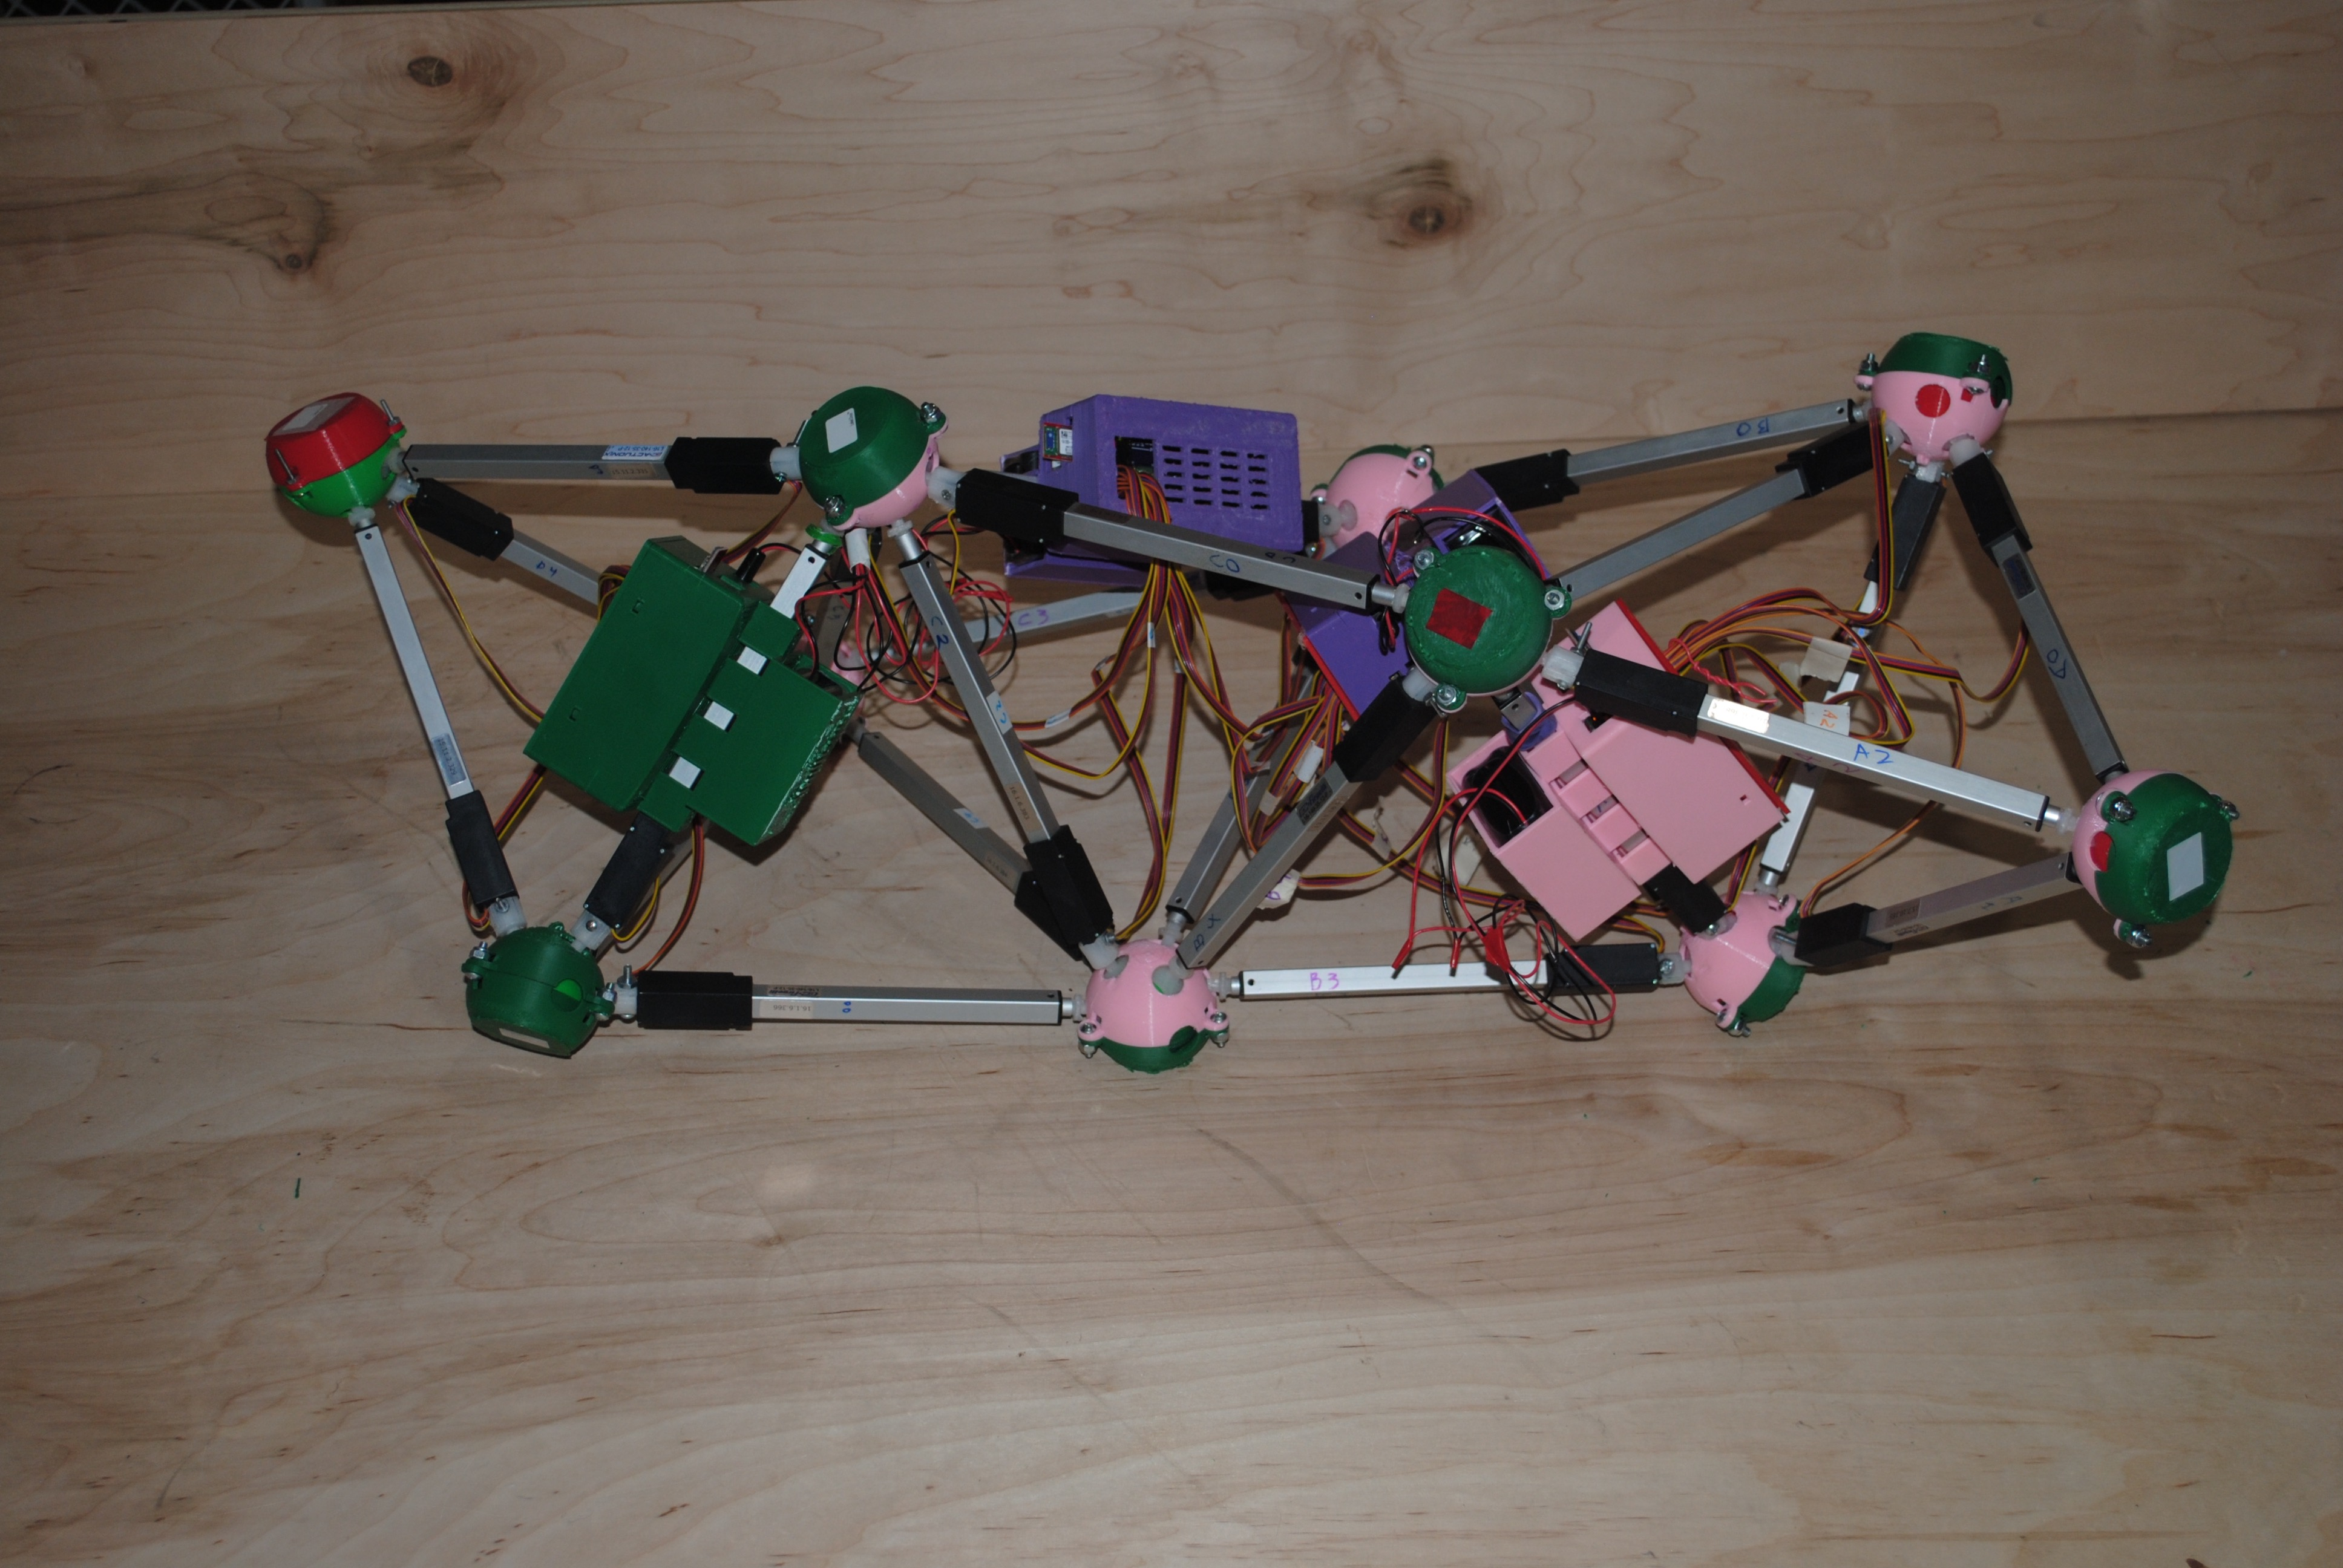
\includegraphics[width=0.4\textwidth]{figures/GlussBotBC.jpg}
     \caption{Glussbot in relaxed, or BC helix configuration}
     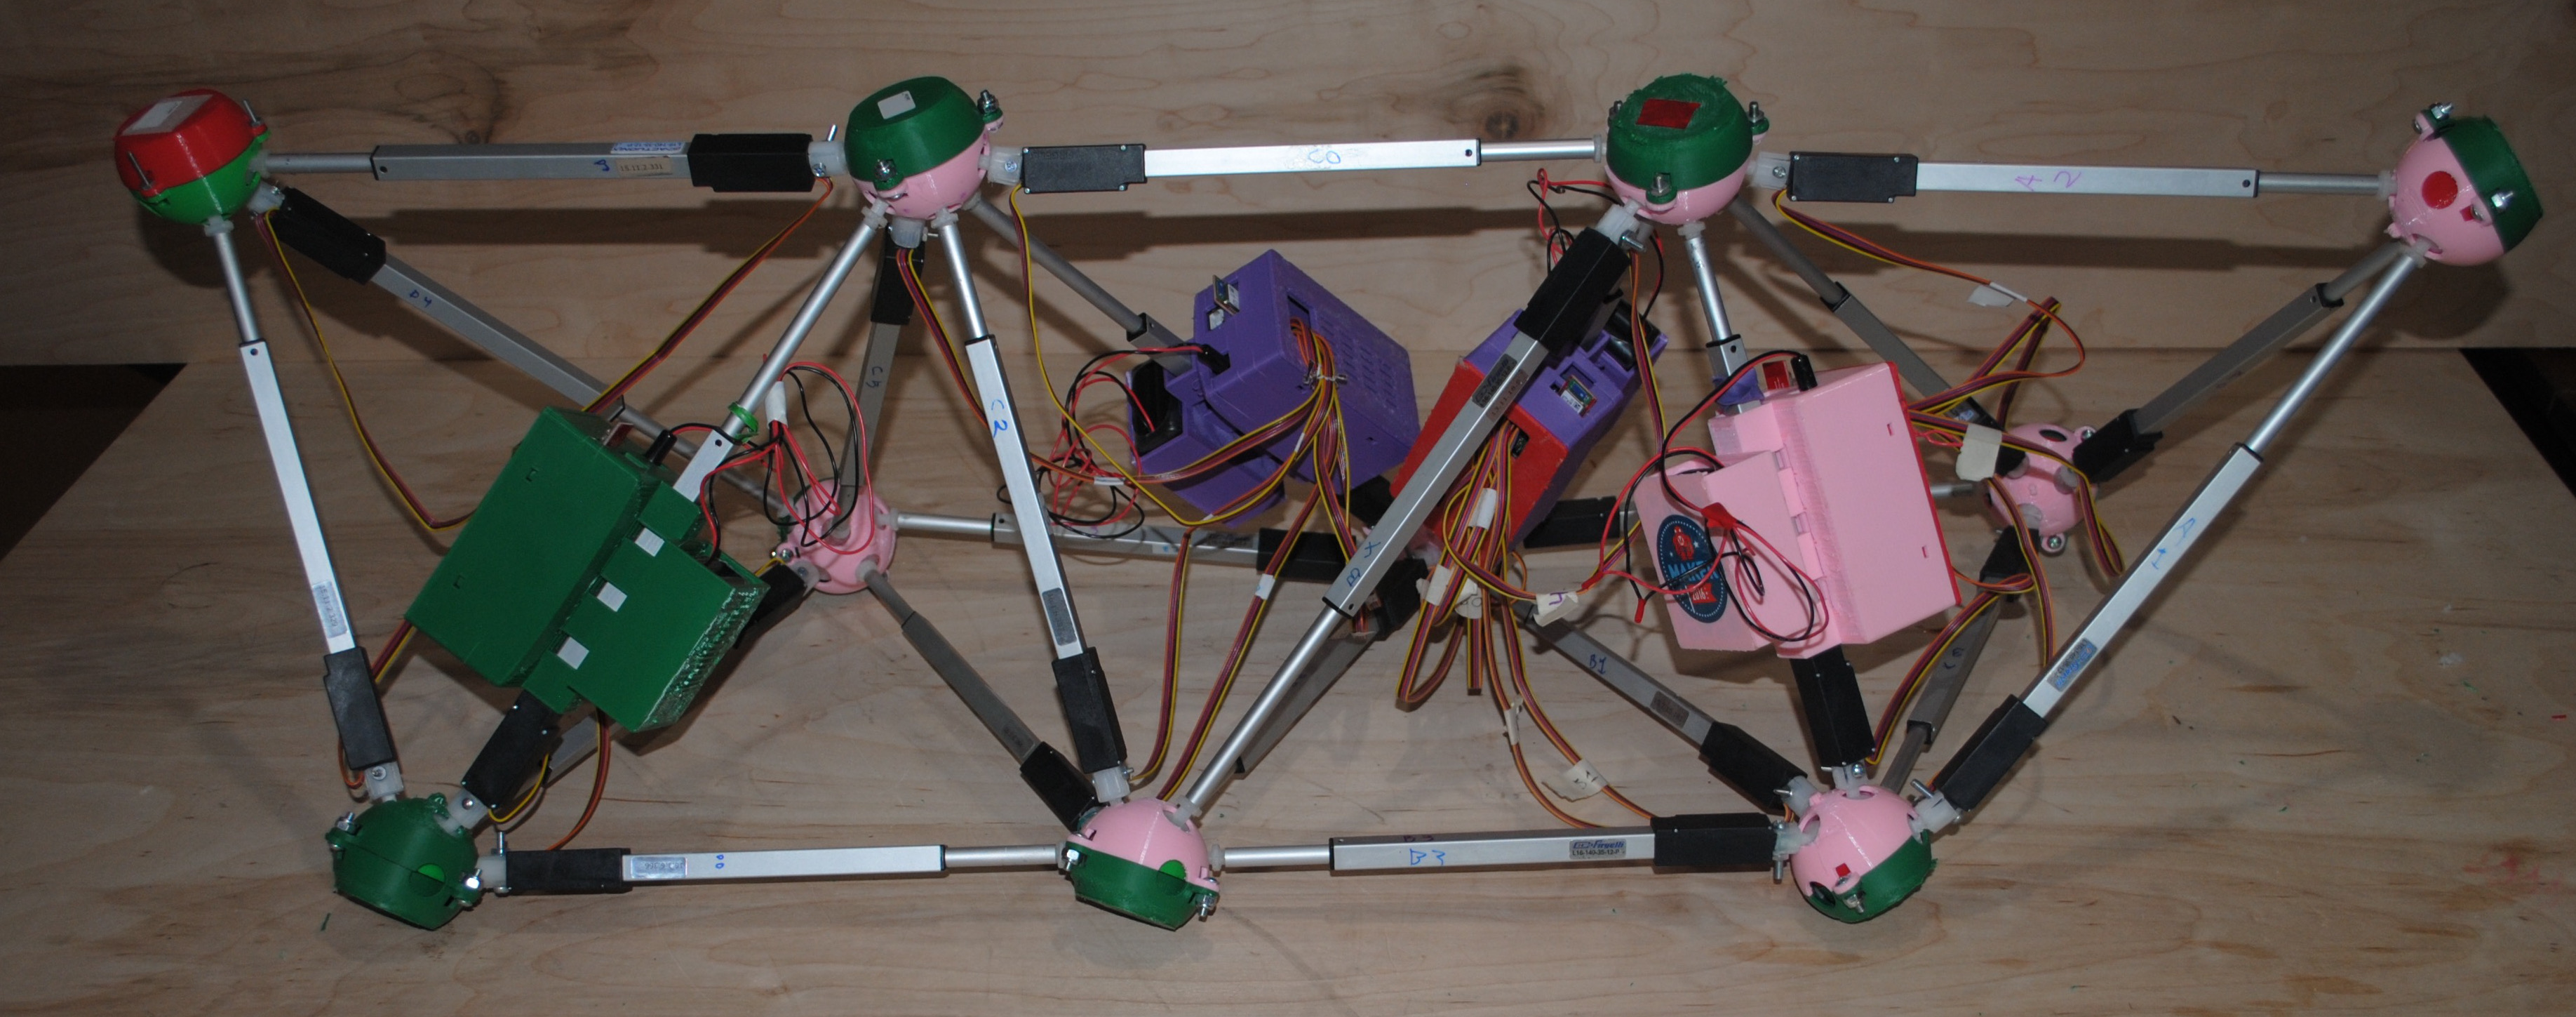
\includegraphics[width=0.4\textwidth]{figures/GlussBotEquitetrabeamCropped.jpg}
     \caption{The Equitetrabream: Fully Untwisted Glussbot}
\end{figure}

\end{proof}

\section{Conclusion}

The BC Helix is the end point of a continuum of tetrahelices, the
other end point being an uncurved tetrahelix with equilateral cross
section, constructed by changing the length of only those members
crossing the outside rails after hopping over the nearest
vertex. Under the condition of miminum maximum length difference of
all members in the system, all such tetrahelices have vertices evenly
spaced along the axis generated by a simple equation.  A mechanical
machine, such as a robot or a variable-geometry truss, that can change
the length of its members, can thus twist and untwist itself by
changing the length of the appropriate members to achieve any point in
the continuum optimally. With a numeric solution, a design may choose
a rotation angle and member lengths to obtain any desired pitch.

\section{Contact and Getting Involved}

The Gluss Project \url{http://pubinv.github.io/gluss/} is part of Public Invention,
a free-libre, open-source research, hardware, and software project that welcomes volunteers.
It is our goal to organize projects for the benefit of all humanity without seeking profit or intellectual property.
To assist, contact \href{mailto:read.robert@gmail.com}{$<$read.robert@gmail.com$>$}.

\bibliographystyle{IEEEtran}
\bibliography{IEEEabrv,gluss}

\end{document}

TODO:

Clean up d_{opt}.

Produce mini table of pitch vs. \rho?

Improve clarity and precision of proofs.

Solve the chirality problem.

Check every step of my derivation at rho = 0 and the BC values.

Found something.  So now the computation of the optimal radii seems slightly better than what we had before.
We have not, however, proven it to be optimal in the ranges involved, but at least we seem to be computing it correctly.

See if we can accurately compute the derivative of two-hop - one-hop and if it is always negative, meaning that
it is always optimal to set one-hop = 1.  The we have a way to compute one-hope.

Remove the weirdly colored diagram.

Add to the rail angle diagram.

Note that Lamba = 16 almost produces a 2-rail helicoid.

When abs(lambda) > 4, we seem to have marked differences in the parameters. Understand why this is and what is causing it.
(it is possible that positive and negative rho values behave very differently?

Note: Would be really nice to have the GUI show you all computed parameters.

Note: Distance is clearly lower on first computations..

Create working toolkit for design/exploration.

Improve code that way, use white background, floor.

Figure out if I am computing something wrong.



Try to compute optimal radius within our context. This would let us assert that we have
an ``optimum'' continuum.  Not worth much to an engineer, but valuable.

Review and continue editing, being careful to introduce concepts in the correct order.

On Rail diagram, add a second tetrahedron, and a second rho.



Make YouTube video.



Possible addtional refrerences and submissions:

Journal of applied geometry seems like a good fit:

http://epubs.siam.org/toc/sjaabq/1/1

According to there editorial board, they welcome mathematcal software and
online resources such as I provie.

This one has a nice editing structure: Metric Geometry is a nice subset:

http://discreteanalysisjournal.com/for-authors

  
http://bit-player.org/2013/tetrahedra-with-a-twist

This is unrelated, but well worth reading:

https://arxiv.org/pdf/1702.06388.pdf

Research Turk's knots
